\normaltrue
\correctiontrue

%\UPSTIidClasse{11} % 11 sup, 12 spé
%\newcommand{\UPSTIidClasse}{12}

%\section{Rotation simple} %\label{B2:12:01}
\exer{Mouvement R  $\star$ \label{B2:13:02}}
\setcounter{numques}{0}
\UPSTIcompetence[2]{C2-05}
\UPSTIcompetence[2]{B2-13}
\index{Compétence C2-05}
\index{Compétence B2-13}
\index{Mécanisme à 1 rotation}
\ifcorrection
\else
\textbf{Pas de corrigé pour cet exercice.}
\fi

\ifprof
\else
Soit le mécanisme suivant. On a $\vect{AB}=R\vect{i_1}$ avec $R=\SI{20}{mm}$. 
\begin{center}
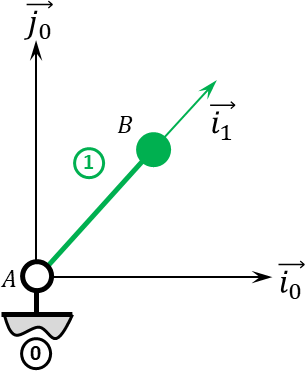
\includegraphics[width=\linewidth]{02_R_01}
\end{center}
\fi

\question{Quel est le mouvement de \textbf{1} par rapport à~\textbf{0}.}
\ifprof
\textbf{1} est en rotation de centre $A$ et d'axe $\vk{0}$ par rapport à \textbf{0}.
\else
\fi

\question{Quelle est la trajectoire du point $B$ appartenant à \textbf{1} par rapport à~\textbf{0}.}
\ifprof
$B$ est est en rotation par rapport à \textbf{0} (cercle de centre $A$ et de rayon $R$).
\else
\fi

\question{Donner l'équation paramétrique de la trajectoire du point $B$, point appartenant à \textbf{1} par rapport à ~\textbf{0}.}
\ifprof

On a $\vect{AB}=R\vi{1}$ $=R\cos\theta \vi{0}+R\sin\theta \vj{0}$. La trajectoire du point $B$ est donc donnée par 
$\left\{ 
\begin{array}{l}
x_B(t) = R\cos\theta (t) \\
y_B(t) = R\sin\theta (t) \\
z_B(t)=0 
\end{array}
\right.$ dans le repère $\repere{A}{i_0}{j_0}{z_0}$.

\else
\fi

\ifprof
\else
\footnotesize
\begin{center}
\begin{tabular}{|p{.9\linewidth}|}
\hline
Indications :
\begin{enumerate}
\item .
\item .
\item $x_B(t) = R\cos\theta (t)$ et $y_B(t) = R\sin\theta (t)$.
\end{enumerate} \\ \hline
\end{tabular}
\end{center}
\normalsize

\begin{flushright}
\footnotesize{Corrigé  voir \ref{B2:13:02}.}
\end{flushright}%
\fi